La sesión analizada contó con un total de 70 senadores,
pertenecientes a 27 partidos políticos, distribuidos del
siguiente modo (figura \ref{fig-distrib-senators}):

\begin{figure}[h!]
\centering
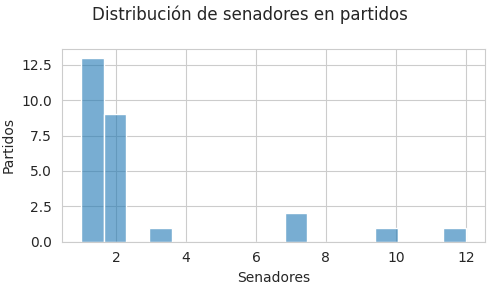
\includegraphics[scale=0.7]{../visualizations/distrib_histplot_senators_parties.png}
\caption{Distribución de senadores en partidos políticos.}
\label{fig-distrib-senators}
\end{figure}

Solo uno de los partidos (Frente de todos) cuenta con 12
senadores; también uno solo (Alianza frente para la victoria) es
representado por 10 senadores; dos partidos (Alianza cambiemos y
Juntos por el cambio) cuentan con 7 senadores, y el resto de los
partidos tienen entre 3, 2 y un senador.
En cuanto a las provincias (24 en total), todas tienen 3 senadores
exceptuando a Tucumán y a La Rioja, que tienen solo 2.

La figura \ref{fig-distrib-vote} nos muestra además que la intención
de voto no guarda una relación unívoca con los partidos a los cuales los
senadores representan. A excepción de los partidos que cuentan con un único
senador, la mayoría es representado con senadores que votaron a favor y senadores
que votaron en contra de la ley para el acceso al aborto. Aquí también
es posible ver que un senador del Frente Justicialista se abstuvo de votar,
mientras que dos senadores, uno de Cambiemos Fuerza Cívica Riojana y uno de
Frente Unidad Justicialista San Luis, estuvieron ausentes en la votación.

\begin{figure}[h!]
\centering
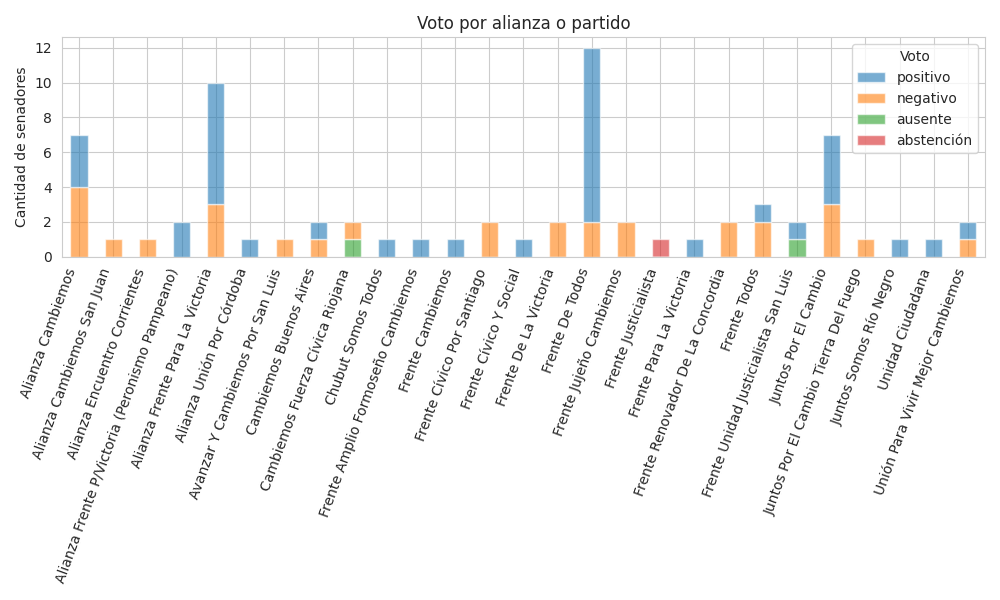
\includegraphics[scale=0.48]{../visualizations/senators_vote_by_party.png}
\caption{Distribución de votos en los distintos partidos políticos.}
\label{fig-distrib-vote}
\end{figure}

Respecto de las intervenciones discursivas, observamos que, en promedio, se emitieron
2.87 discursos por senador, con un desvío estándar de 6.23 y una mediana de 1, coincidente además
con la moda, lo que nos indicaría que se trata de una distribución asimétrica a derecha.
Estas medidas de centralidad incluyen a 9 senadores que no intervinieron en
la sesión, 7 de ellos votaron en contra de la despenalización del aborto; uno, a favor,
y uno estuvo ausente durante la votación. La figura \ref{fig-distrib-speech} muestra esta
distribución global y también discriminada por intención de voto.
Al desagregar los datos según elección en la votación, vemos que las abstenciones no presentan
dispersión y su media se ubica en el valor 1. Esto se debe a que solo un senador
se abstuvo de votar y, a su vez, solo emitió un discurso.
Una situación similar se da en las ausencias, donde también se observa un único discurso.
Pero dado que dos senadores estuvieron ausentes, la media se ubica hacia el valor 0.5 y
el desvío, hacia el 0.7.
En cuanto a los votos positivos y negativos, ambos presentan una moda de 1, pero los negativos
exhiben una media y un desvío estándar mayor que los positivos: $3.03\pm8.43$ \textit{versus} 
$2.92\pm4.26$, respectivamente. Ambos casos presentan obsrvaciones atípicas, pero en los votos
negativos estos casos muestran valores más extremos, por lo que la media y el desvío se
ven influenciados y adoptan también valores más altos.

\begin{figure}[h!]
    \centering
    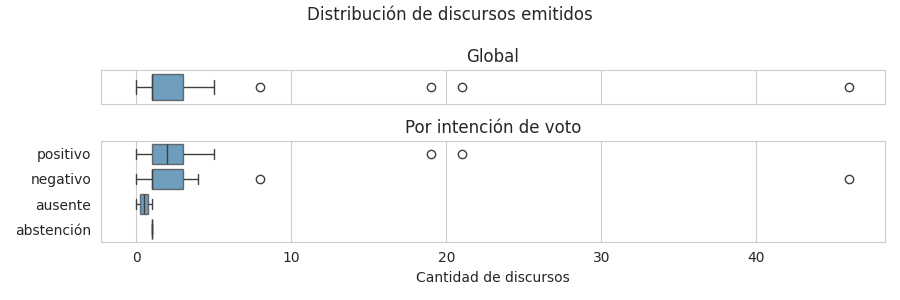
\includegraphics[scale=0.5]{../visualizations/speech_by_vote.png}
    \caption{Distribución de votos en los distintos partidos políticos.}%
    \label{fig-distrib-speech}
\end{figure}

Por último, al hacer foco en la longitud de los discursos pronunciados, vemos que su
distribución varía dependiendo de si los medimos en \textit{tokens} totales o únicos.
Un \textit{token} es una secuencia de caracteres que queremos considerar como un
grupo\footnote{\citet*{bird2009natural}}. Aquí este grupo constituye lo que denominamos
`palabra'. En promedio, los discursos emitidos tienen 418 palabras, con un desvío
estándar de 714 palabras; la mediana es de 11 y la moda, de 7. Sin embargo, estas medidas
reflejan las palabras totales utilizadas en cada intervención, sin considerar si se repiten
o no: cada ocurrencia de una palabra cuenta, sin importar si ya fue pronunciada en el mismo
discurso. Es por eso que, a fines comparativos, se tomaron también las medidas de centralidad
de los \textit{tokens} únicos, las cuales mostraron una media de 161 palabras por discurso
con un desvío de 245, una mediana de 11 y una moda de 1. La figura \ref{fig-distrib-tokens}
refleja este contraste. Como es posible observar, si bien en ambos casos los discursos
muestran \textit{outliers} respecto de su longitud, cuando esta se mide en palabras
totales, presenta una mayor cantidad de casos atípicos con valores más extremos que
al medirla en \textit{tokens} únicos. En este último caso, un
$20\percentsign$ de los registros son \textit{outliers}, de los cuales solo el
$17\percentsign$ constituyen casos extremos, mientras que, al considerar
el total de palabras, un $22\percentsign$ de los datos resultan atípicos y,
de ellos, el $32\percentsign$ son extremos\footnote{Para este análisis se utilizó el
test de Tukey, que toma el rango intercuartil o \textit{IQR} (\textit{Q3-Q1}, donde
\textit{Q1} refiere al primer cuartil y \textit{Q3}, al terceo) y considera
valores atípicos leves a aquellos que se encuentran entre
$Q1 - (1.5 * IQR) < x < Q3 - (1.5 * IQR)$ y como extremos a los que están entre
$Q1 - (3 * IQR) < x < Q3 - (3 * IQR)$.}.

\begin{figure}[h!]%
    \centering%
    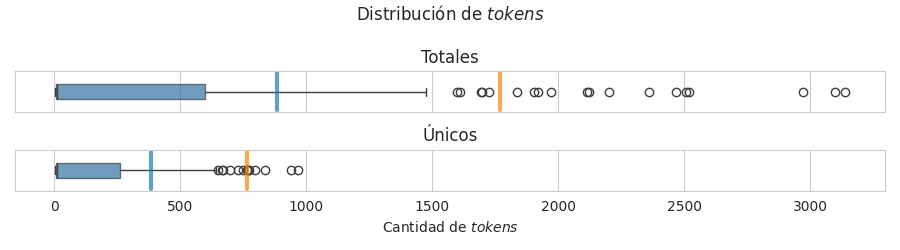
\includegraphics[scale=0.5]{../visualizations/distrib_tokens.png}%
    \caption{Distribución de \textit{tokens} totales y únicos en los discursos pronunciados. En ambos gráficos,
    la línea azul indica el límite a partir del cual una observación se considera atípica leve
    ($IQR*1.5$) y la naranja, el límite a partir del cual se la considera atípica extrema ($IQR*3$).}%
    \label{fig-distrib-tokens}%
\end{figure}%


%\begin{table}[ht]
%\centering
%\begin{tabular}{ |c|c|c|c|c| }
%    \hline
%    Voto & Media & Desvío & Mediana & Moda \\
%    \hline\hline
%    Abstención & 1.00 & 0.00 & 1.00 & 1 \\
%    \hline
%    Ausente & 0.50 & 0.71 & 0.50 & 0 \\
%    \hline
%    Negativo & 3.03 & 8.43 & 1.00 & 1 \\
%    \hline
%    Positivo & 2.92 & 4.26 & 2.00 & 1 \\
%    \hline
%\end{tabular}
%\caption{Medidas de centralidad de la cantidad de discursos emitidos}
%\label{table-tokens}
%\end{table}
